\documentclass[12pt, twoside]{article}
\usepackage[letterpaper, margin=1in, headsep=0.5in]{geometry}
\usepackage[english]{babel}
\usepackage[utf8]{inputenc}
\usepackage{amsmath}
\usepackage{amsfonts}
\usepackage{amssymb}
\usepackage{tikz}
%\usetikzlibrary{quotes, angles}

\usepackage{graphicx}
\usepackage{enumitem}
\usepackage{multicol}

\usepackage{fancyhdr}
\pagestyle{fancy}
\fancyhf{}
\renewcommand{\headrulewidth}{0pt} % disable the underline of the header

\fancyhead[RE]{\thepage}
\fancyhead[RO]{\thepage \\ Name: \hspace{3cm}}
\fancyhead[L]{BECA / Dr. Huson / 10th Grade Geometry\\* 10 May 2019}

\begin{document}
\subsubsection*{Homework: Triangle relationships}
 \begin{enumerate}

   \item Given two parallel lines that intersect a transversal,  $\overleftrightarrow{DE} || \overleftrightarrow{BC}$. $m\angle ABC =3x-5$ and $m\angle BDE=6x+5$. \\[0.5]
   Find $m\angle ADE$.\\[2cm]
     \begin{tikzpicture}[scale=1.1]
       \draw [<->, thick] (-1,0)--(0,0)--(4,0);
       \draw [<->, thick] (-0.5,-0.5)--(3,3)--(3.5,3.5);
       \draw [<->, thick] (1,2)--(5, 2)--(5.5,2);
       \draw [fill] (3,3) circle [radius=0.05] node[above left]{$A$};
       \draw [fill] (5, 2) circle [radius=0.05] node[below]{$E$};
       \draw [fill] (2,2) circle [radius=0.05] node[above left]{$D$};
       \draw [fill] (0,0) circle [radius=0.05] node[above left]{$B$};
       \draw [fill] (3,0) circle [radius=0.05] node[below]{$C$};
     \end{tikzpicture} \vspace{4cm}

     \item Given  $\triangle EFG$ with $\overline{EF}$ extended to $A$. If $m\angle F=38^\circ$ and $m\angle AEG=133^\circ$, what is $m\angle EGF$?
       \begin{center}
         \begin{tikzpicture}%[scale=0.7]
           \draw [thick](0,0)node[below]{$A$}--
             (2,0)node[below]{$E$}--
             (8,0)node[below]{$F$}--
             (4,3)node[above]{$G$} --(2,0);
         \end{tikzpicture}
       \end{center}

\newpage
  \item Given two vertical angles as shown, $m \angle 1 = 5x+5$, $m \angle 2 = 7x-17$.\\[0.5cm]
  Find $m \angle 1$.\\[0.5cm] For full credit find the $m\angle 2$ as a check.
    \begin{flushright}
    \begin{tikzpicture}[scale=.7]
      \draw [<->, thick] (0,-1.5)--(10,1.5);
      \draw [<->, thick] (2,3.5)--(7,-3.5);
      \node at (3,.4){1};
      \node at (6,-.6){2};
      %\draw [fill] (0,0) circle [radius=0.05] node[below]{$P$};
      %\draw [fill] (6,0) circle [radius=0.05] node[below]{$R$};
      %\draw [fill] (3,0) circle [radius=0.05] node[below]{$Q$};
    \end{tikzpicture}
    \end{flushright}
  \vspace{3cm}

  \item Given $\overrightarrow{BA} \perp \overrightarrow{BC}$, $m \angle ABD = 5x+47$, and $m \angle DBC = 2x+22$. Find $m \angle DBC$. \\[0.5cm]
  For full credit, show the check using both angle measures.
    \begin{flushleft}
    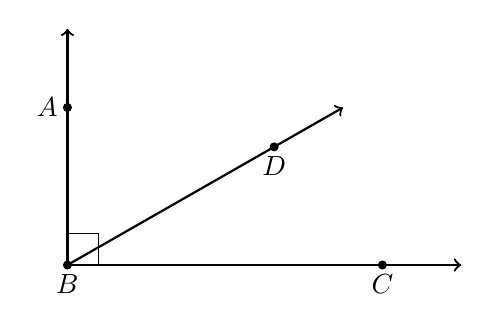
\begin{tikzpicture}[scale=1]
      \draw [<->, thick] (0,3)--(0,0)--(5,0);
      \draw [->, thick] (0,0)--(3.5, 2);
      \draw [-, thin] (0, 0.4)--(0.4, 0.4)--(0.4, 0);
      %\node at (3,.4){1};
      %\node at (6,-.6){2};
      \draw [fill] (0,0) circle [radius=0.05] node[below]{$B$};
      \draw [fill] (0,2) circle [radius=0.05] node[left]{$A$};
      \draw [fill] (4,0) circle [radius=0.05] node[below]{$C$};
      \draw [fill] (2.625, 1.5) circle [radius=0.05] node[below]{$D$};
    \end{tikzpicture}
    \end{flushleft}

\newpage
  \item $A(2,10)$ is one endpoint of $\overline{AB}$. The segment's midpoint is $M(5,7)$. Find the other endpoint, $B$. \vspace{4cm}

  \item In the diagram below, $\triangle ABC$ has vertices with coordinates $A(1,3)$, $B(8,4)$ and $C(4, 7)$.
    \begin{center} %4 quadrant regents grid
      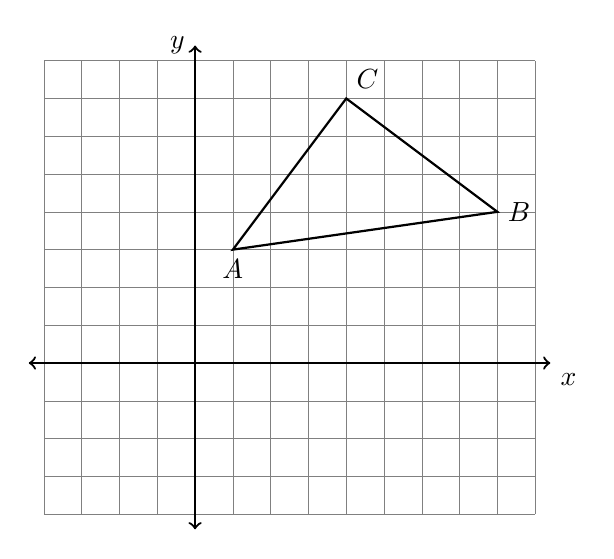
\begin{tikzpicture}[scale=.48]
        \draw [help lines] (-4,-4) grid (9,8);
        \draw [thick, <->] (-4.4,0) -- (9.4,0) node [below right] {$x$};
        \draw [thick, <->] (0,-4.4)--(0,8.4) node [left] {$y$};
        \draw [thick]
          (1,3)node[below]{$A$}--
          (8,4) node[right]{$B$}--
          (4,7) node[above right]{$C$}--cycle;
        %\draw [fill] (-1,2) circle [radius=0.1] node[above left] {$A$};
        %draw [fill] (8, -4) circle [radius=0.1] node[below right] {$C$};
      \end{tikzpicture}
    \end{center}
    Find the length of each side of $\triangle ABC$, showing that it is isosceles and not equilateral.\\[0.5cm]
      \begin{tabular}{c|c|c}
        $AC=$ & $BC=$ & $AB=$ \\
        $\sqrt{(x_C-x_A)^2+(y_C-y_A)^2}$ & $\sqrt{(x_C-x_B)^2+(y_C-y_B)^2}$ & $ \sqrt{(x_B-x_A)^2+(y_B-y_A)^2}$ \\
        & & \\
        & & \\
      \end{tabular}

\newpage
  \begin{multicols}{2}
    [\item A translation maps triangle $ABC$ onto triangle $DEF$.] \vspace{0.5cm}
      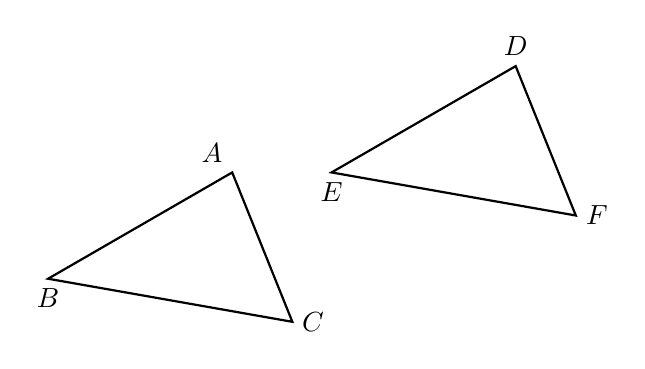
\begin{tikzpicture}[scale=0.9]
        \coordinate [label=above left:$A$](A) at (30:3);
        \coordinate [label=below:$B$](B) at (0, 0);
        \coordinate [label=right:$C$](C) at (-10:3.5);
        \draw [thick] (A)--(B)--(C)--cycle;

        \draw [thick, xshift=4cm, yshift=1.5cm] (30:3) node[above]{$D$}--
        (0,0) node[below]{$E$}--
        (-10:3.5) node[right]{$F$}--cycle;
      \end{tikzpicture}\\
      Fill in the blank with the corresponding object.
      \begin{enumerate}
        \item $A \rightarrow$ \rule{2cm}{0.15mm} \vspace{0.3cm}
        \item $\angle ABC \cong$ \rule{2cm}{0.15mm}
        \item \rule{2cm}{0.15mm} $\cong \overline {EF}$
      \end{enumerate}
    \end{multicols} \vspace{1cm}

   \item The vertices of $\triangle JKL$ have the coordinates $J(-4,-2)$, $K(-1,-1)$, and $L(-2,3)$, as shown below. \\[0.5cm]
   Apply a translation of $(x,y) \rightarrow (x+7, y+4)$ to $\triangle JKL$ and then reflect the image across the $x$-axis. Draw both images $\triangle J'K'L'$ and $\triangle J''K''L''$ on the set of axes below, labeling the vertices.
   \begin{center}
     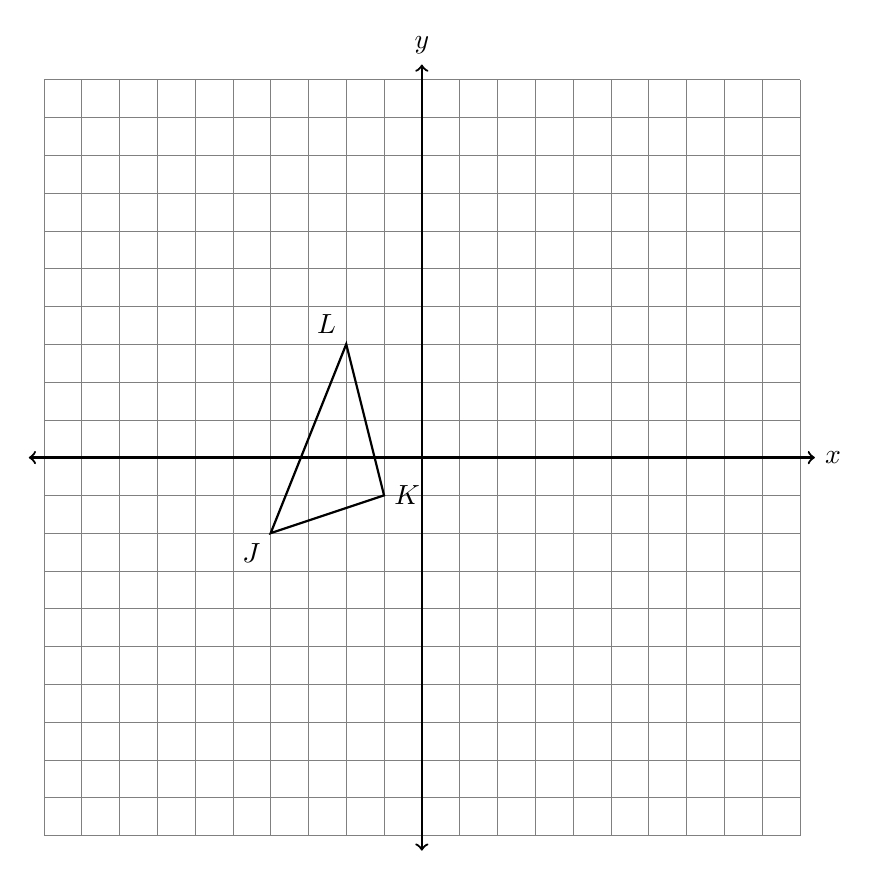
\begin{tikzpicture}[scale=.48]
       \draw [help lines] (-10,-10) grid (10,10);
       \draw [thick, <->] (-10.4,0) -- (10.4,0) node [right] {$x$};
       \draw [thick, <->] (0,-10.4)--(0,10.4) node [above] {$y$};

       \draw [thick]
       (-4,-2) node[below left] {$J$}--
       (-1,-1) node[right] {$K$}--
       (-2,3) node[above left] {$L$}--
       cycle;
     \end{tikzpicture}\\[0.5cm]
  \end{center}

\end{enumerate}
\end{document}
